

\documentclass{beamer}
 
\usepackage[utf8]{inputenc}
\usepackage{pgfpages}
\usepackage{array}

\setbeameroption{hide notes}
 
%Information to be included in the title page:
\title[Automated Design of Probabilistic Selection Methods for EA's]
{The Automated Design of Probabilistic Selection Methods for Evolutionary Algorithms}
 
\author[Richter, Samuel \& Tauritz, Daniel] % (optional, for multiple authors)
{Samuel Richter (snr359@mst.edu) \\Daniel Tauritz (dtauritz@acm.org)}
 
\institute % (optional)
{
  Natural Computation Laboratory\\
  Department of Computer Science\\
  Missouri University of Science and Technology\\
  Rolla, Missouri 65409
}
 
\date{ECADA @ GECCO, July 2018}
 
\usetheme{Copenhagen}
 
\begin{document}
 
	\frame{\titlepage}
	
	\begin{frame}
		\frametitle{Introduction}
		
		\begin{itemize}
			 \item<1-|alert@1> For Evolutionary Algorithms (EA's), the method of parent/survival selection has a significant impact on performance
			 \item<2-|alert@2> Manual Tuning of selection strategy can lead to improvement but is still limited to existing/conventional methods
			 \item<3-|alert@3> Generation of new selection methods, specialized to particular problems, can improve performance further
		\end{itemize}
	\end{frame}
	
	\begin{frame}
		\frametitle{Overview}
			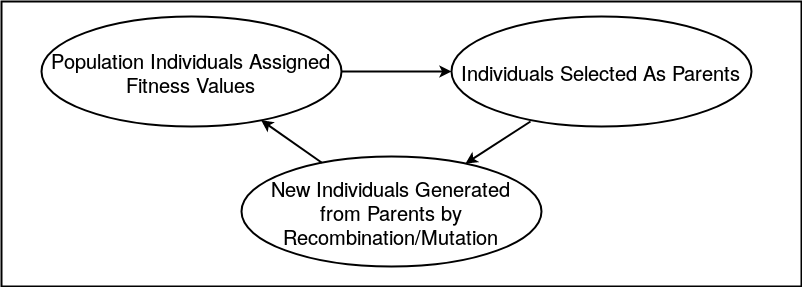
\includegraphics[width=1\textwidth]{ea_cycle}
			\\
			Parent Selection and Survival Selection both strongly influence how genes survive in the population
	\end{frame}
	
	\begin{frame}
		\frametitle{Overview}
			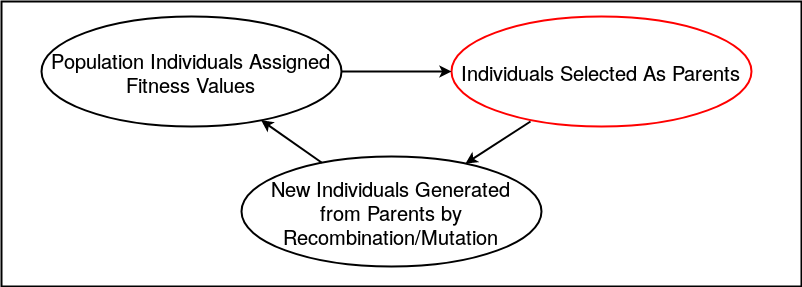
\includegraphics[width=1\textwidth]{ea_cycle_highlight}
			\\
			We wish to develop a customized selection function specialized to a particular problem class. For this study, we chose to specialize parent selection, while keeping survival selection static.
			\note{Our choice to improve parent selection, rather than survival selection or both simultaneously, was mostly arbitrary for the sake of proof-of-concept}
	\end{frame}
	
	\begin{frame}
		\frametitle{Overview}
		\begin{itemize}
			 \item<1-> Objective: use a Hyper-Heuristic to generate a selection function for a particular EA operating on a particular problem class
			 \item<2-|alert@2> Step 1: define a representation for selection functions to form a search space
	 			 \note[item]<2>{We are generating selection functions by defining a search space containing new selection functions, then searching through that space}
			 \item<3-|alert@3> Step 2: explore this space and determine the quality of the selection functions to find the best one
		\end{itemize}	
	\end{frame}	
	
	\begin{frame}
		\frametitle{Representation}
		\begin{itemize}
			 \item<1-|alert@1> A straightforward way to represent selection functions would be to employ a Turing-complete algorithm space that takes a population as input, and returns an individual or pool of individuals
			 \note[item]<1>{This is a straightforward representation, but not the only possible straightforward representation}
			 \item<2-|alert@2> However, the space of Turing-complete algorithms is large and complex, making it difficult to search through 
			 	\note[item]<2>{The Turing-complete space has the additional challenge of ensuring that the algorithms generated are valid selection functions}
		
		\end{itemize}	
	\end{frame}			
	
	
	\begin{frame}
		\frametitle{Representation}
		
		\begin{itemize}
			 \item<1-|alert@1> We instead represent selection functions as mathematical functions, which determine the relative probability that any given individual is selected
			 \item<2-|alert@2> This function uses an individual's fitness, fitness ranking, the population size, and the sum of population fitness as inputs, and uses typical mathematical operators (+, -, *, /) as well as a step function
			 	\note[item]<2>{We chose these particular terminals and operators because all of the conventional selection functions we tested against (fitness-proportional, k-tournament, etc.) can be represented by them. \\The step function, which is formally the ``Heaviside Step Function'', in this case, is a binary function. When the left operand is greater than or equal to the right operand, the function returns 1; otherwise, it returns 0}
			 \item<3-|alert@3> The function is evaluated for each individual, and a weighted random selection is performed, using the function output as the weight for each individual
			 \item<4-|alert@4> An additional boolean variable controls whether selection is performed with replacement
				 \note[item]<4>{When the boolean variable is True, individuals may be selected more than once within a single generation. When it is False, an individual can only be selected once per generation}
			 
		
		\end{itemize}
	\end{frame}
	
	\begin{frame}
		\frametitle{Representation}
		A selection function is represented by a mathematical function (encoded in a parse tree), and the boolean variable.
		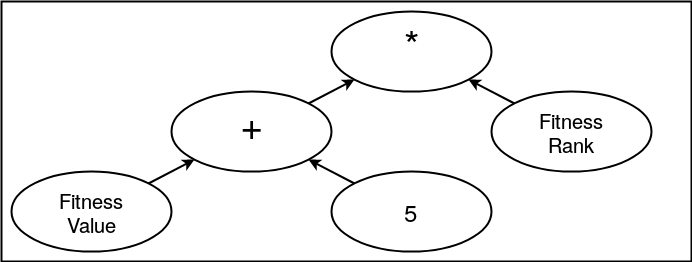
\includegraphics[width=\textwidth]{example_adpsea_no_replacement_bit}
	\end{frame}
	
	\begin{frame}
		\frametitle{Representation - Psuedocode}
		\begin{columns}
			\column{0.4\textwidth}
				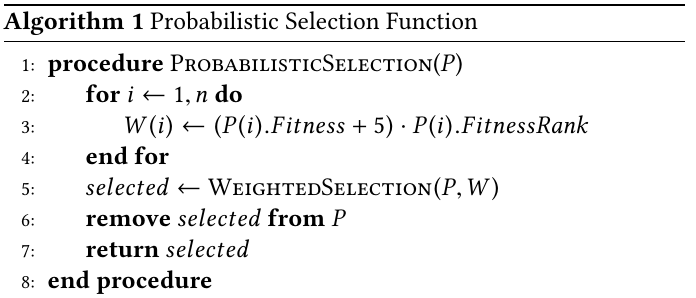
\includegraphics[width=0.45\paperwidth]{adpsea_code_1}
			\column{0.55\textwidth}
				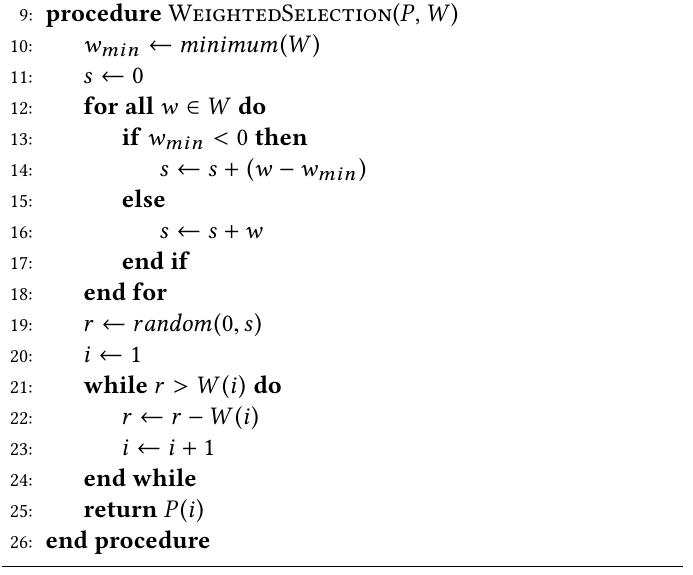
\includegraphics[width=0.45\paperwidth]{adpsea_code_2}
		\end{columns}
		\note{Here we show the psuedocode of the generated selection function. It is composed of two parts: an assignment of function outputs to population members (line 3) and a weighted selection being performed using the function outputs as weights. "FitnessRank" refers to the individual's fitness ranking in the population, where 1 is the ranking of the lowest-fitness individual and \textit{n} is the ranking of the highest-fitness individual, in a population of \textit{n} individuals. This particular code is generated by the example given earlier (the exact portions of code affected are highlighted in the next slide).}
	\end{frame}
	
	\begin{frame}
		\frametitle{Representation - Psuedocode}
		\begin{center}
			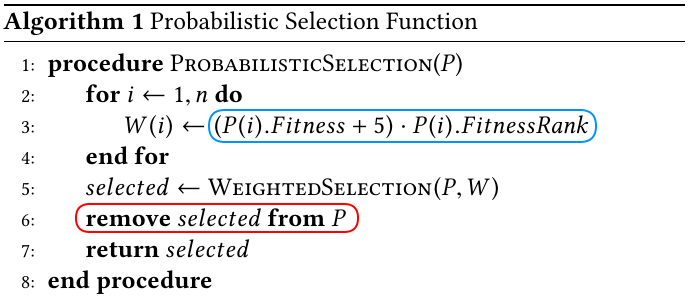
\includegraphics[width=0.9\paperwidth]{adpsea_code_1_highlight}
		\end{center}
		\note{Here we show the first part of the algorithm in more detail. The portion of code highlighted in blue is the portion changed by a different function tree. The line highlighted in red is present if the "replacement" bit is set to True, and removed if the bit is set to False.}
	\end{frame}
	
	\begin{frame}
		\frametitle{Representation - Psuedocode}
		\begin{center}
			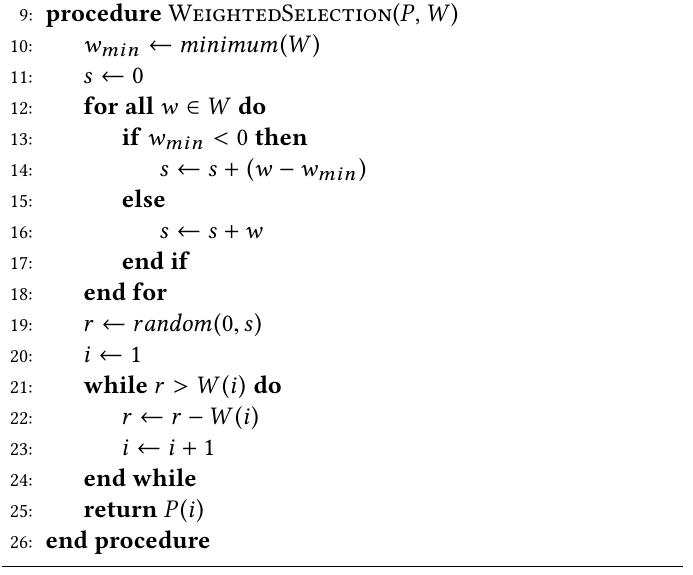
\includegraphics[width=0.6\paperwidth]{adpsea_code_2}
		\end{center}
		\note{Here we show the second part of the algorithm in more detail. It is identical to a standard roulette-wheel fitness proportional selection, except for the weights for each individual. Instead of using the fitness values directly, the output of the selection function is used. Note that a typo exists in our published paper, where line 22 is incorrectly "r = r + W(i).}
	\end{frame}	
	 
	\begin{frame}
		\frametitle{Representation - Example}
		Selection Function: $P(selection) \propto (Fitness + 5) * FitnessRank$
		\begin{table}
			\begin{tabular}{ m{5cm} | c | c | c | c }
				Population Member & 1 & 2 & 3 & 4  \\
				\hline
				Fitness & 300 & 250 & 200 & 350  \\
				& & & & \\ 
				& & & & \\ 
				& & & & \\ 
			\end{tabular}
		\end{table}		
	\end{frame} 

	\begin{frame}
		\frametitle{Representation - Example}
		Selection Function: $P(selection) \propto (Fitness + 5) * FitnessRank$
		\begin{table}
			\begin{tabular}{ m{5cm} | c | c | c | c }
				Population Member & 1 & 2 & 3 & 4  \\
				\hline 
				Fitness & 300 & 250 & 200 & 350  \\
				Fitness Rank (least to greatest) & 3 & 2 & 1 & 4  \\
				& & & & \\ 
				& & & & \\ 
			\end{tabular}
		\end{table}		
	\end{frame}
	 
	\begin{frame}
		\frametitle{Representation - Example}
		Selection Function: $P(selection) \propto (Fitness + 5) * FitnessRank$
		\begin{table}
			\begin{tabular}{ m{5cm} | c | c | c | c }
				Population Member & 1 & 2 & 3 & 4  \\
				\hline 
				Fitness & 300 & 250 & 200 & 350  \\
				Fitness Rank (least to greatest) & 3 & 2 & 1 & 4  \\
				$(Fitness + 5) * FitnessRank$ & 915 & 510 & 205 & 1420  \\
				& & & & \\ 
			\end{tabular}
		\end{table}		
	\end{frame}
	 
	\begin{frame}
		\frametitle{Representation - Example}
		Selection Function: $P(selection) \propto (Fitness + 5) * FitnessRank$
		\begin{table}
			\begin{tabular}{ m{5cm} | c | c | c | c }
				Population Member & 1 & 2 & 3 & 4  \\
				\hline 
				Fitness & 300 & 250 & 200 & 350  \\
				Fitness Rank (least to greatest) & 3 & 2 & 1 & 4  \\
				$(Fitness + 5) * FitnessRank$ & 915 & 510 & 205 & 1420  \\
				P(selection) & 0.3 & 0.167 & 0.067 & 0.466  \\ 
			\end{tabular}
		\end{table}		
	\end{frame}
	
	\begin{frame}
		\frametitle{Representation - Example}
		Selection Function: $P(selection) \propto (Fitness + 5) * FitnessRank$
		\begin{table}
			\begin{tabular}{ m{5cm} | c | c | c | c }
				Population Member & 1 & 2 & 3 & 4  \\
				\hline
				Fitness & 300 & 250 & 200 & 350  \\
				Fitness Rank (least to greatest) & 3 & 2 & 1 & 4  \\
				$(Fitness + 5) * FitnessRank$ & 915 & 510 & 205 & 1420  \\
				P(selection) & 0.3 & 0.167 & 0.067 & 0.466  \\ 
				\hline \hline
				$Fitness+100*PopulationSize$ & 700 & 650 & 600 & 750  \\
				P(selection) & 0.259 & 0.241 & 0.222 & 0.278  \\
				
			\end{tabular}
		\end{table}
		\note{Here we provide an example of the function output and P(selection) for a second function}		
	\end{frame}		
	
	\begin{frame}
		\frametitle{Representation - Example}
		Selection Function: $P(selection) \propto (Fitness + 5) * FitnessRank$
		\begin{table}
			\begin{tabular}{ m{5cm} | c | c | c | c }
				Population Member & 1 & 2 & 3 & 4  \\
				\hline
				Fitness & 300 & 250 & 200 & 350  \\
				Fitness Rank (least to greatest) & 3 & 2 & 1 & 4  \\
				$(Fitness + 5) * FitnessRank$ & 915 & 510 & 205 & 1420  \\
				P(selection) & 0.3 & 0.167 & 0.067 & 0.466  \\ 
				\hline \hline
				$Fitness+100*PopulationSize$ & 700 & 650 & 600 & 750  \\
				P(selection) & 0.259 & 0.241 & 0.222 & 0.278  \\ 				
				\hline \hline
				$step(Fitness, 300) * Fitness$ & 300 & 0 & 0 & 350  \\
				P(selection) & 0.461 & 0.0 & 0.0 & 0.549  \\ 
			\end{tabular}
		\end{table}		
		\note{Here we provide a third function as another example}
	\end{frame}	
	
	\begin{frame}
		\frametitle{Representation - Example}
		Selection Function: $P(selection) \propto (Fitness + 5) * FitnessRank$
		\begin{table}
			\begin{tabular}{ m{5cm} | c | c | c | c }
				Population Member & 1 & 2 & 3 & 4  \\
				\hline
				Fitness & 300 & 250 & 200 & 350  \\
				Fitness Rank (least to greatest) & 3 & 2 & 1 & 4  \\
				$(Fitness + 5) * FitnessRank$ & 915 & 510 & 205 & 1420  \\
				P(selection) & 0.3 & 0.167 & 0.067 & 0.466  \\ 
				\hline \hline
				$Fitness+100*PopulationSize$ & 700 & 650 & 600 & 750  \\
				P(selection) & 0.259 & 0.241 & 0.222 & 0.278  \\ 				
				\hline \hline
				$step(Fitness, 300) * Fitness$ & 300 & 0 & 0 & 350  \\
				P(selection) & 0.461 & 0.0 & 0.0 & 0.549  \\ 
				\hline \hline
				P(fitness-proportional) & 0.273 & 0.227 & 0.182 & 0.318\\
				\hline \hline
				P(fitness-ranking) & 0.3 & 0.2 & 0.1 & 0.4\\
			\end{tabular}
		\end{table}		
		\note{Here we show fitness proportional and fitness rank selection for comparison as well}
	\end{frame}		
	 
	\begin{frame}
		\frametitle{Representation}
		Different selection functions, including conventional and our evolved selection functions, offer different probability distributions over the population
		\begin{center}
			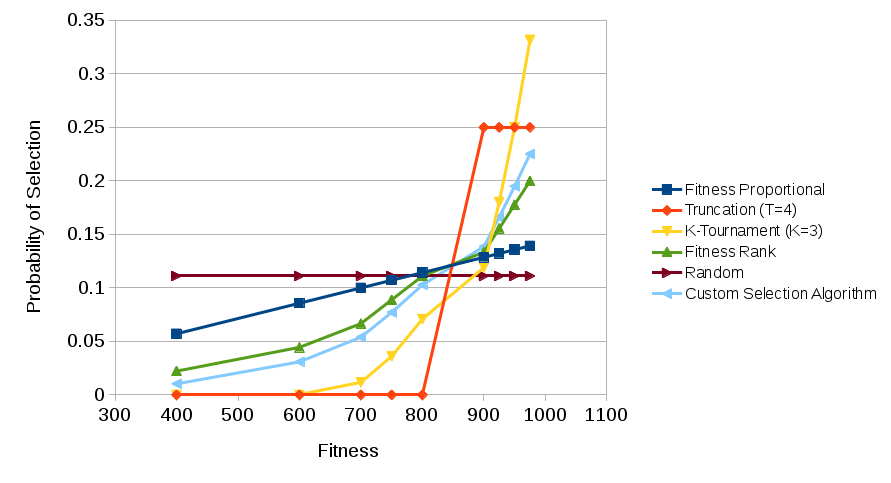
\includegraphics[height=0.65\paperheight]{selection_chances}
		\end{center}
		\note{This line graph shows the probability of selected for each individual in a population of 9 individuals, with fitness values of 400, 600, 700, 750, 800, 900, 925, 950, and 975. The ``Custom Selection Algorithm'' is the same one used in previous examples, $P(selection) \propto (Fitness + 5) * FitnessRank$}
	\end{frame}
	
	\begin{frame}
		\frametitle{Representation}
		Many conventional selection functions can be represented in this format
		\\
		\begin{center}
			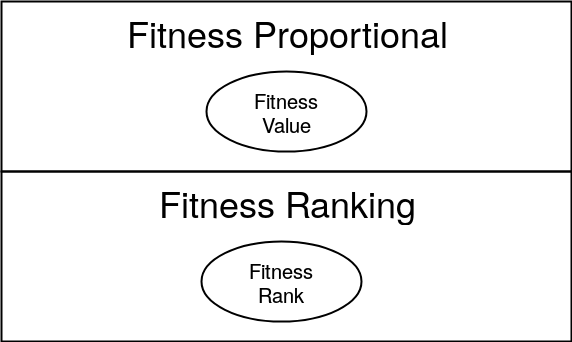
\includegraphics[width=\paperheight]{example_selections_1}
		\end{center}
		\note{Variations of Fitness-Value and Fitness-Rank selection are seen fairly often in the population. Variations of truncation and K-tournament are less common.}
	\end{frame}
	
	\begin{frame}
		\frametitle{Representation}
		Many conventional selection functions can be represented in this format
		\\
		\begin{center}
			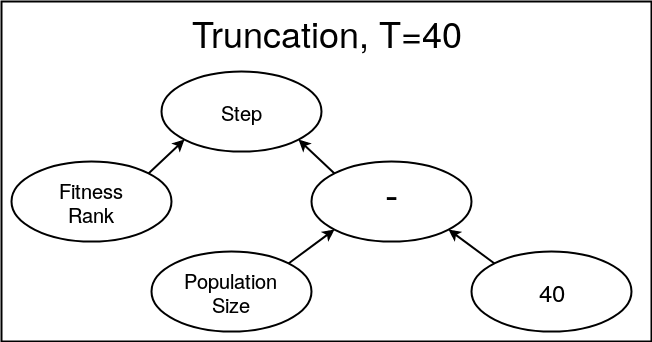
\includegraphics[width=\paperheight]{example_selections_2}
		\end{center}
		\note{Variations of Fitness-Value and Fitness-Rank selection are seen fairly often in the population. Variations of truncation and K-tournament are less common.}
	\end{frame}	
	
	\begin{frame}
		\frametitle{Representation}
		Many conventional selection functions can be represented in this format
		\\
		\begin{center}
			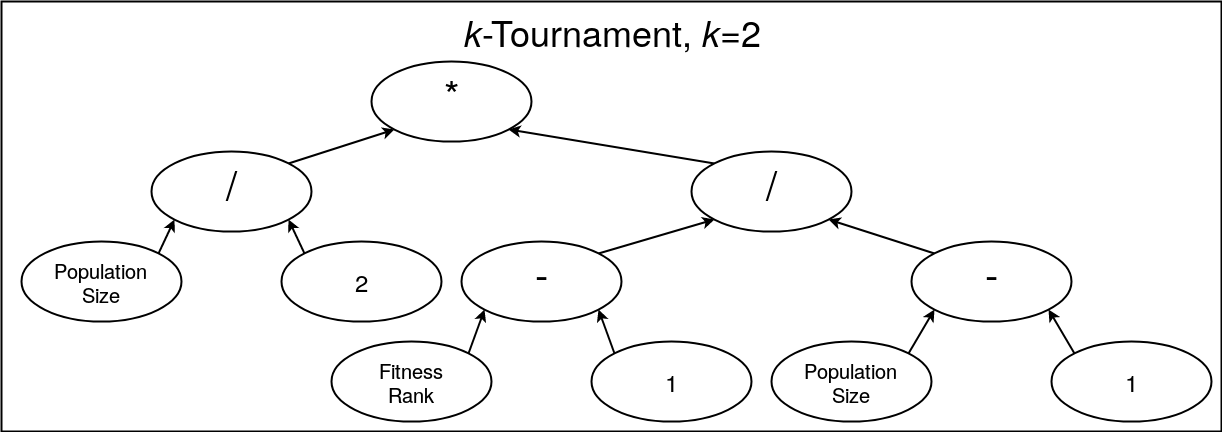
\includegraphics[width=\paperheight]{example_selections_3}
		\end{center}
		\note{Variations of Fitness-Value and Fitness-Rank selection are seen fairly often in the population. Variations of truncation and K-tournament are less common.}
	\end{frame}	
	
	\begin{frame}
		\frametitle{Representation}
		
		\begin{itemize}
			 \item<1-|alert@1> This format allows us a more manageable search space of selection functions, while also being robust enough to represent both conventional selection functions and a wide variety of new selection functions
			 \item<2-|alert@2> In addition, we can guarantee that all functions in this space are valid selection functions
			 \item<3-|alert@3> We cannot guarantee that all possible selection functions can be represented in this format, but this is an acceptable tradeoff for the more easily-searchable space of selection functions
		\end{itemize}
	\end{frame}	
	
	\begin{frame}
		\frametitle{Meta-EA}
		
		\begin{itemize}
			 \item<1-|alert@1> We use Koza-style GP to evolve the trees representing the selection strategies
			 \item<2-|alert@2> Each strategy is evaluated by running a sub-level EA utilizing that strategy on a fixed set of benchmark instances from the NK-Landscape problem class, with N=40 and K=8
				\note{We chose N=40 and K=8 to generate problem classes that were difficult enough to warrant the use of an EA, but easy enough that a performance benefit could be gained by varying the selection function only.}			 
			 \item<3-|alert@3> After the meta-EA is run, the selection strategies are tested for generalization on a separate set of ``testing'' instances from the same problem class
		\end{itemize}
	\end{frame}
	
	\begin{frame}
		\frametitle{Meta-EA Parameters}
		\begin{table}
			\small
			\begin{tabular}{ c | c | }
			    Parameter& Value\\
			    \hline \hline
			    Population Size & 50 \\
			    \hline
			    Offspring Size & 50\\
			    \hline
			    Evaluation Count & 2500\\
			    \hline
			    Max GP-Tree Initialization Depth & 3\\
			    \hline
			    Parent Selection & \textit{k}-tournament, \textit{k}=10 \\
			    \hline
			    Survival Selection & Random\\
			    \hline
			    Mutation & Subtree Regeneration\\
			    \hline
			    Crossover & Subtree Crossover\\
			    \hline
			    Parsimony Pressure Coefficient & 1\\
			    \hline
			    Mutation Rate & 0.1\\
			    \hline
			    Training Instances & 20 \\
			    \hline
			    Runs per Training Instance & 3 \\
			    \hline
			    Testing Instances & 50 \\
			    \hline
			    Runs per Testing Instance & 100 \\
			    \hline
			    Range for Constant Terminals & [-100, 100]\\
			    \hline
			    Range for Random Terminals & [-100, 100]\\
			\end{tabular}
		\end{table}
	\end{frame}
	
	\begin{frame}
		\frametitle{Base EA Parameters}
		\begin{table}
			\small
			\begin{tabular}{ c | c | }
			    Parameter & Value\\
			    \hline \hline		    
			    Population Size & 100 \\
			    \hline
			    Offspring Size & 20\\
			    \hline
			    Genome Length (N) & 40 \\
			    \hline
			    Locus Length (K) & 8\\
			    \hline
			    Locus Minimum Value & 0\\
			    \hline
			    Locus Maximum Value & 8\\
			    \hline
			    Parent Selection & (evolved in Meta-EA)\\
			    \hline
			    Survival Selection & Random \\
			    \hline
			    Termination Criteria & Convergence \\
			    \hline
			    Generations to Convergence & 25\\
			    \hline
			    Mutation & Random Bit Flip \\
			    \hline
			    Mutation Rate & 0.05\\
			    \hline
			    Crossover & Uniform Crossover\\
			\end{tabular}
		\end{table}
		\note{At the time the paper was written, the parameters were human-chosen arbitrarily, but now, iRace is used to find good parameters to test against.}
	\end{frame}	
	
	\begin{frame}
		\frametitle{Results - Comparison with Conventional Selection Methods}
		\begin{columns}
			\column{0.3\textwidth}
				The final best selection strategy evolved by the Meta-EA outperformed all conventional selection strategies tested on 94\% of the 50 testing instances.
			\column{0.7\textwidth}
				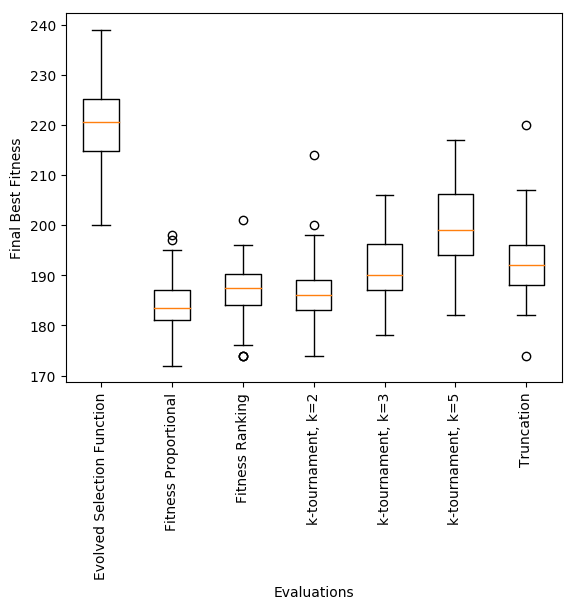
\includegraphics[height=0.7\paperheight]{nk_landscape_boxplot}	
		\end{columns}
		\note{The boxes on these box-and-whisker extend from first to third quartile, and indicate the median. The top and bottom whiskers extend to the most extreme data points within $Q3+1.5*IQR$ and $Q1-1.5IQR$, respectively, where IQR is the interquartile range. Data points indicated with circles are outside the whiskers and considered outliers}
	\end{frame}
	
	\begin{frame}
		\frametitle{Results - Final Best Evolved Selection Strategy}
		\begin{center}
			$P(selection) \propto PopulationSize / ((FitnessRank/(FitnessRank-PopulationSize))-PopulationSize)$, selecting \textbf{with} replacement
			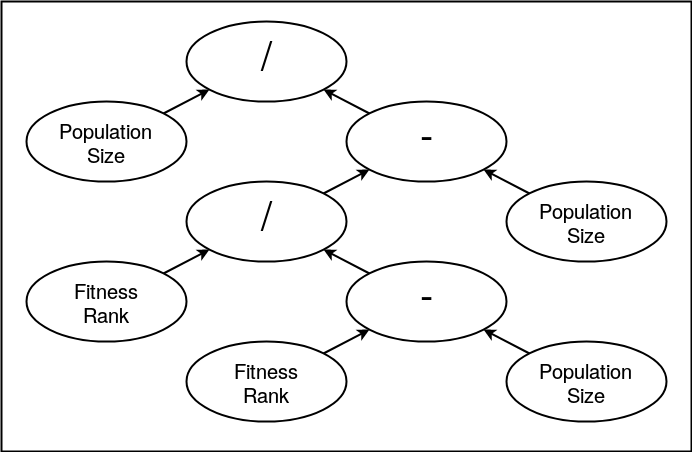
\includegraphics[height=0.60\paperheight]{adpsea_final_no_replacement_bit}		
			\\
			The Final Best Evolved Selection Strategy
		\end{center}
	\end{frame}
	
	\begin{frame}
		\frametitle{Results - Final Best Evolved Selection Strategy}
		\begin{center}
			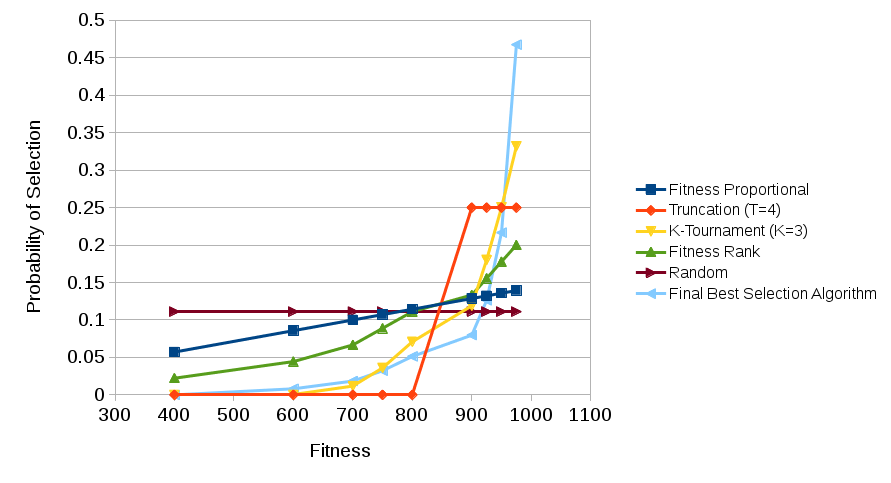
\includegraphics[width=\textwidth]{selection_chances_with_final}\\
			$P(selection) \propto PopulationSize / ((FitnessRank/(FitnessRank-PopulationSize))-PopulationSize)$, selecting \textbf{with} replacement
		\end{center}
		\note{Here we show the selection chances again, but with a line corresponding to the final evolved best function, and how it would select from the example population given (note that this example population was selected arbitrarily, not part of any experiment, and that the behavior shown may not correspond to what the evolution was trending toward).}
	\end{frame}	
	
	\begin{frame}
		\frametitle{Limitations}
			\begin{itemize}
			\item<1-|alert@1> The Meta-EA can require large amounts of computing resources, especially if the sub-level EA is computationally expensive
			\item<2-|alert@2> The evolved selection methods are static, and do not adapt/self-adapt as the evolution progresses
			\item<3-|alert@3> The sub-level EA uses static parameters for population size, number of offspring generated, mutation rate, and survival selection
			\end{itemize}
	\end{frame}
	
	\begin{frame}
		\frametitle{Future Work}
		\begin{itemize}
			\item<1-|alert@1> Investigate tuning of survival selection, as well as parent selection
			\item<2-|alert@2> Tune selection strategies for other problems, including real-world problems
			\item<3-|alert@3> Evolve dynamic/self-adjusting selection strategies
			\item<4-|alert@4> Evolve selection strategies for an EA using dynamic/adaptive parameters, rather than static/fixed parameters
			\item<5-|alert@5> Investigate other weighted selection strategies apart from a weighted random selection.
			\item<6-|alert@6> Investigate systems to encourage more diversity in parents selected, beyond a binary ``with/without replacement'' setting
		\end{itemize}
	\end{frame}
	
	\begin{frame}
		\frametitle{``Take Home Message''}
			\begin{itemize}
				\item<1-|alert@1> An EA running on a problem class can gain a performance benefit with a selection function specialized to that problem class (with all other parameters unchanged)
				\item<2-|alert@2> A Meta-EA Hyper-heuristic can be used to search through a space of selection functions to find one that significantly outperforms common selection  functions for a particular problem class
			\end{itemize}
	\end{frame}


 
\end{document}

